%\renewcommand{\theequation}{\theenumi}
%\begin{enumerate}[label=\thesubsection.\arabic*.,ref=\thesubsection.\theenumi]
%%\begin{enumerate}[label=\arabic*.,ref=\thesection.\theenumi]
%\numberwithin{equation}{enumi}

\item Draw a circle of diameter 6.1

\item With the same centre $\vec{O}$,  draw two circles of radii 4 and 2.5
\\
\solution


All input values required to plot Fig. \ref{constr/52/tab:table1} are given in Table \ref{constr/52/tab:table1} as shown below

\begin{table}[!ht]
\begin{center}
    \resizebox{\columnwidth}{!}{
\begin{tabular}{ | m{2cm} | m{1.5cm}| m{2cm} | m{1.5cm} |} 
\hline
& Symbols & Circle1 & Circle2 \\
\hline
Centre & $\vec{O}$ & \myvec{0\\0} & \myvec{0\\0} \\ 
\hline
Radius & $r_{1}$,$r_{2}$ & 2.5 & 4 \\ 
\hline
Polar coordinate & $\vec{C}_{1}$,$\vec{C}_{2}$ & 2.5\myvec{\cos \theta\\  \sin \theta} & 4\myvec{\cos \theta\\  \sin \theta} \\
\hline
Angle & $\theta$ & 0-2$\pi$ & 0-2$\pi$ \\
\hline
\end{tabular}
    }
\end{center}
\caption{Input values}
\label{constr/52/tab:table1}
\end{table}


\begin{figure}[!ht]
\centering
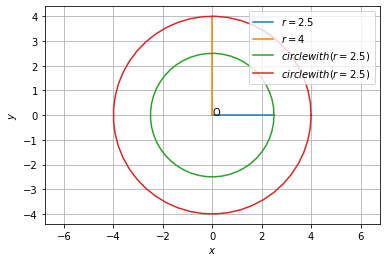
\includegraphics[width=\columnwidth]{solutions/52/Figure3.png}
\caption{Concentric circles with centre as origin and radii 2.5 and 4 respectively}
\label{constr/52/fig:circle}	
\end{figure}



\item Draw a circle with centre $\vec{B}$ and radius 6.  If $\vec{C}$ be  a point 10 units  away from its 
centre, construct the pair of tangents $AC$ and $CD$ to the 
circle.
\item Draw a circle of radius 3 and any two of its diameters.  Draw the ends of these diameters. What figure do you get?
\item Let $\vec{A}$ and $\vec{B}$ be the centres of two circles of equal radii 3 such that each one of them passes through the centre of the other.  Let them intersect at $\vec{C}$ and $\vec{D}$.  Is $AB \perp CD$?
\\
\solution
The centers and radii of the two circles without any loss of generality are given in Table \ref{constr/55/tab:table1}
%
\begin{table}[!ht]
\begin{center}
\begin{tabular}{ | m{2cm} | m{2cm} | m{2cm} |} 
\hline
 & Circle 1 & Circle 2 \\
\hline
Centre  & $\vec{A}$=\myvec{0\\0} & $\vec{B}$=\myvec{3\\0} \\ 
\hline
Radius & $r_{1}=r_{2}=3$  \\ 
\hline
\end{tabular}
\end{center}
\caption{Input values}
\label{constr/55/tab:table1}

\end{table}

% The choice for $\vec{A}$ and $\vec{B}$ is valid as:
% \begin{align}
% \norm{\vec{B}-\vec{A}} = \norm{\vec{A}-\vec{B}}=\norm{\vec{B}}  = 3 \quad \brak{\because \vec{A}=0}
% \end{align}

Let 
\begin{align}
\vec{u}=\myvec{\cos \theta\\  \sin \theta},  \theta \in \sbrak{0,2\pi}.
\end{align}

Then on Circle 1  and Circle 2 are  given by 
\begin{align}
\vec{x}&=\vec{A}+r\vec{u}
\\
\vec{x}&=\vec{B}+r\vec{u}
\end{align}

Fig. \ref{constr/55/fig:circle} is plotted using the above equations.
%
\begin{figure}[!ht]
\centering
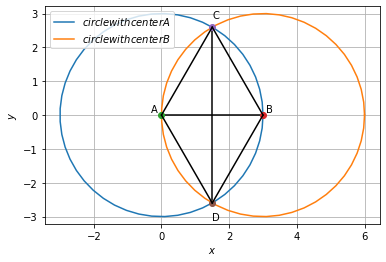
\includegraphics[width=\columnwidth]{solutions/55/Figures/figure3.png}
\caption{Circles with their points of intersection}
\label{constr/55/fig:circle}	
\end{figure}
Fig. \ref{constr/55/fig:circle} 

The general equation of Circle 1 is given by 
\begin{align}
    \norm{\vec{x}-\vec{A}}^2 &= r^2
    \\
\vec{x}^{\top}\vec{x} - 2\vec{A}^{\top}\vec{x} + \norm{\vec{A}}^2 -r_{1}^2 &= 0\label{constr/55/eq:14}
\end{align}
Similarly, for Circle 2,
\begin{align}
\vec{x}^{\top}\vec{x} - 2\vec{B}^{\top}\vec{x} + \norm{\vec{B}}^2 -r_{2}^2 = 0\label{constr/55/eq:15}
\end{align}
Subtracting \eqref{constr/55/eq:15} from \eqref{constr/55/eq:14},
\begin{align}
2\vec{B}^{\top}\vec{x}=\norm{\vec{B}}^2
\\
\myvec{1&0}\vec{x}=\frac{3}{2}
\end{align}
which can be expressed as
\begin{align}
\vec{x} &=\frac{1}{2}\myvec{3\\ 0} + \lambda \myvec{0\\1}\label{constr/55/eq:19}\\
&=\vec{q}+\lambda\vec{m} \text{ where}\label{constr/55/eq:20}\\
\vec{q}&=\myvec{1.5\\ 0},
\vec{m}=\myvec{0\\1}
\end{align}
Substituting \eqref{constr/55/eq:20} in \eqref{constr/55/eq:14}
\begin{align}
\norm{\vec{x}}^2=r^2\quad \brak{\because \vec{A}=0}
\\
\norm{\vec{q}+\lambda\vec{m}}^2=r^2\\
(\vec{q}+\lambda \vec{m})^{\top}(\vec{q}+\lambda \vec{m})=r^2\\
\implies \vec{q}^{\top}(\vec{q}+\lambda \vec{m})+\lambda \vec{m}^{\top}(\vec{q}+\lambda \vec{m})=r^2
\\
\implies \norm{\vec{q}}^2+\lambda\vec{q}^{\top}\vec{m}+\lambda\vec{m}^{\top}\vec{q}+\lambda^2\norm{\vec{m}}^2=r^2
\\
\implies \norm{\vec{q}}^2+2\lambda\vec{q}^{\top}\vec{m}+\lambda^2\norm{\vec{m}}^2=r^2 
% \\
% \implies \lambda(\lambda\norm{\vec{m}}^2+2\vec{q}^{\top}\vec{m})=r^2-\norm{\vec{q}}^2\\
% \implies\lambda^2\norm{\vec{m}}^2=9-\norm{\vec{q}}^2
\\
\implies \lambda=\pm \sqrt{\frac{9-\norm{\vec{q}}^2}{\norm{\vec{m}}^2}} \quad \because \vec{q}^{\top}\vec{m} = 0
% \lambda^2=6.75\\
% \lambda=+\sqrt{6.75},-\sqrt{6.75}
\end{align}
Substituting the value of $\lambda$ in \eqref{constr/55/eq:20},
\begin{align}
%\vec{x}=\vec{q}+\lambda\vec{m}\\
\vec{C}&=\vec{q}+\lambda\vec{m}\\
\vec{D}&=\vec{q}-\lambda\vec{m} \\
\implies (\vec{A}-\vec{B})^{\top}(\vec{C}-\vec{D})
&=2\myvec{-3&0}\myvec{0\\\sqrt{6.75}}
\\
&=0
\\
\implies AB\perp CD
\end{align}


% We have $\vec{C}$ and $\vec{D}$ as points of intersection and $r_{1}=r_{2}$.So,
% \begin{align}
% \norm{\vec{C}-\vec{A}}^2 = \norm{\vec{C}-\vec{B}}^2
% \end{align}
% \begin{align}
% \implies(\vec{C}-\vec{A})^{\top}(\vec{C}-\vec{A})=(\vec{C}-\vec{B})^{\top}(\vec{C}-\vec{B})
% \\
% \implies \vec{A}^{\top}\vec{C}-\vec{B}^{\top}\vec{C}=\vec{C}^{\top}\vec{B}-\vec{C}^{\top}\vec{A}+\norm{\vec{A}}^2-\norm{\vec{B}}^2 
% \end{align}
% \begin{align}
% \implies2\times \vec{A}^{\top}\vec{C}-2\times\vec{B}^{\top}\vec{C}=\norm{\vec{A}}^2-\norm{\vec{B}}^2 \label{constr/55/eq:1}
% \end{align}
% Similarly,using:
% \begin{align}
% \norm{\vec{D}-\vec{A}}^2 = \norm{\vec{D}-\vec{B}}^2
% \end{align}
% We get:
% \begin{align}
% 2\times \vec{A}^{\top}\vec{D}-2\times\vec{B}^{\top}\vec{D}=\norm{\vec{A}}^2-\norm{\vec{B}}^2 \label{constr/55/eq:2}
% \end{align}

% Subtracting equation \ref{constr/55/eq:2} from equation \ref{constr/55/eq:1}:
% \begin{align}
% 2\times(\vec{A}^{\top}-\vec{B}^{\top})(\vec{C}-\vec{D})=0
% \\
% \implies (\vec{A}-\vec{B})^{\top}(\vec{C}-\vec{D})=0
% \\
% \implies AB\perp CD
% \end{align}


\item Construct a tangent to a circle of radius 4 units from a point on the concentric circle of radius 6 
units.
\\
\solution 
The given information is summarised in Table \ref{constr/56/tab}.
\begin{table}[!ht]
\begin{center}
    \resizebox{\columnwidth}{!}{
\begin{tabular}{ | c | c| c| c |} 
\hline
& Symbols & Circle1 & Circle2 \\
\hline
Centre & $\vec{O}$ & \myvec{0\\0} & \myvec{0\\0} \\ 
\hline
Radius & $r_{1}$,$r_{2}$ & 4 & 6\\ 
\hline
\end{tabular}
}
\end{center}
\caption{}
\label{constr/56/tab}
\end{table}
See Fig. \ref{fig:constr/56/Tangent}. Let P be a point on Circle 2 with radius 6.  Then 
\begin{align}
\vec{P} = \myvec{6\\0}
\end{align}
Let $PQ$ and $PR$  be tangents from point $\vec{P}$ on circle with radius 6 to the points $\vec{Q}$ and $\vec{R}$ on circle with radius 4 .
% \begin{align}
% \because OQ \perp QP,
% \end{align}
Now,
\begin{align}
(\vec{O}-\vec{Q})^T (\vec{Q}-\vec{P}) &= 0 \quad \brak{\because OQ \perp QP }
% \\
% \vec{Q}^T(\vec{Q}-\vec{P}) &= 0 \quad \brak{\because \vec{O}=\myvec{0\\0}}
% \\
% \vec{Q}^T \vec{Q} - \vec{Q}^T \vec{P} &= 0  
% \\
% \norm{\vec{Q}}^2 &= \vec{Q}^T \vec{P}
% \\
% \norm{\vec{Q}}^2 &= \vec{P}^T \vec{Q}  \quad \brak{\because \vec{Q}^T \vec{P} = \vec{P}^T \vec{Q}}
\\
\implies \vec{P}^T \vec{Q} &= 16 \quad \brak{\because \norm{\vec{Q}}^2 = 16}
% \\
% \myvec{6&0} \vec{Q} &= 16 \quad \brak{\because \vec{P} = \myvec{6\\0} }
\\
\text{or, }\myvec{1&0} \vec{Q} &= \frac{8}{3}
\\
\implies \vec{Q} &= \myvec{\frac{8}{3}\\0} + \lambda \myvec{0\\1} \label{constr/56/2.0.11} 
\\
&=\vec{q}+\lambda\vec{m}
\\
\text{where }\vec{q}&=\myvec{\frac{8}{3}\\ 0},\vec{m}=\myvec{0\\1}
\end{align}
We know,
\begin{align}
\norm{\vec{q}+\lambda\vec{m}}^2&=r_1^2
\\
(\vec{q}+\lambda \vec{m})^T(\vec{q}+\lambda \vec{m})&=r_1^2
\\
\lambda^2&=\frac{r_1^2-\norm{\vec{q}}^2}{\norm{\vec{m}}^2}
\\
\lambda &= \pm 2.98
\end{align}

Substituting the above in \eqref{constr/56/2.0.11},
%
\begin{align}
\vec{Q}=\myvec{\frac{8}{3}\\2.98},
\vec{R}=\myvec{\frac{8}{3}\\-2.98}
\end{align}
The circels as well as the tangents are plotted in Fig.     \ref{fig:constr/56/Tangent}
%
\begin{figure}[ht]
    \centering
    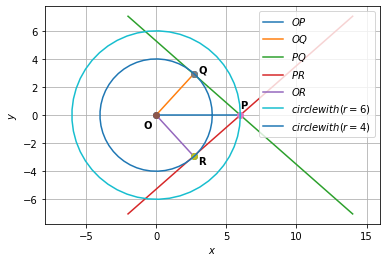
\includegraphics[width=\columnwidth]{solutions/circle/56/TANGENT.png}
    \caption{Tangent lines to circle of radius 4 units.}
    \label{fig:constr/56/Tangent}
\end{figure}    





\item Draw a circle of radius 3 units. Take  two points $\vec{P}$ and $\vec{Q}$ on one of its extended 
diameter each at a distance of 7 units from its centre. Draw tangents to the circle from these two points 
$\vec{P}$ and $\vec{Q}$.
\\
\solution Take the diameter to be on the $x$-axis.
\item Draw a pair of tangents to a circle of radius 5 units which are inclined to each other at an angle of 
$60^{\degree}$.
\\
\solution The tangent is perpendicular to the radius.
\item Draw a line segment $AB$ of length 8 units. Taking $\vec{A}$ as centre, draw a circle of radius 4 units 
and taking $\vec{B}$ as centre, draw another circle of radius 3 units. Construct tangents to each circle from 
the centre of the other circle.
\\
\solution Let
\begin{align}
\vec{A} = \myvec{0 \\ 0}, \vec{B} = \myvec{8 \\ 0}.
\end{align}
\item Let ABC be a right triangle in which $a = 8, c = 6$ and $\angle B = 90^{\degree}$.  $BD$ is the 
perpendicular from $\vec{B}$ on $AC$ (altitude). The circle through $\vec{B}, \vec{C}, \vec{D}$ (circumcircle of $\triangle BCD$) is drawn.  Construct the 
tangents from $\vec{A}$ to this circle.
%\\
%\solution Since $\angle BDC = 90\degree$, $BC$ is the diameter of the circumcircle of $\triangle BCD$. Since $AB \perp BC$ and $BC$ is the diameter, $AB$ is a tangent to the circumcircle of $\triangle BCD$.  Let $\vec{O}$ be the centre of the circle.  The point of contact is obtained by rotating $\vec{B}$ by $\theta = 2\angle BAO$. Thus, if 
%\begin{align}
%\vec{B} &= \myvec{0 \\ 0}, \vec{C} = \myvec{a \\ 0},
%\\
%\vec{O} &= \frac{1}{2}\myvec{a \\ 0}
%\end{align}

\item Draw a circle with centre $\vec{C}$ and radius 3.4.  Draw any chord.  Construct the perpendicular bisector of the chord and examine if it passes through $\vec{C}$
%\end{enumerate}
%
%\item Form the differential equation represeting the family of curves given by 
%\begin{align}
%\vec{x}^T \myvec{1 & 0 \\ 0 & 2} \vec{x} -\myvec{2a & 0}\vec{x} = 0,
%\end{align}
%%
%where $a$ is an arbitrary constant.
%%
%\item Form the differntial equation of the family of circles in the first quadrant which touch the coordinate axes.
%\end{enumerate}
